% ------------------------------------------------------------------------
% AMS-LaTeX Paper ********************************************************
% ------------------------------------------------------------------------
% Submitted:      Dec 15 2003
% Final Version:  
% Accepted:       
% ------------------------------------------------------------------------
% This is a journal top-matter template file for use with AMS-LaTeX.
%%%%%%%%%%%%%%%%%%%%%%%%%%%%%%%%%%%%%%%%%%%%%%%%%%%%%%%%%%%%%%%%%%%%%%%%%%

%\documentclass{tran-l}
%\documentclass[twocolumn]{amsart}
%\documentclass[]{amsart}
%\documentclass[]{sig-alternate}
\documentclass[]{acm_proc_article-sp}
%\documentclass[]{llncs}


%\documentclass[]{prentcsmacro}

%\usepackage[active]{srcltx} % SRC Specials for DVI Searching
\usepackage{url}
\usepackage[pdf]{pstricks}
\usepackage{pstricks-add, pst-grad, pst-plot}
\usepackage[tiling]{pst-fill}
\usepackage{verbatim}
\usepackage{tikz}
\usetikzlibrary{matrix,arrows}
\usetikzlibrary{backgrounds}
\usetikzlibrary{decorations.pathmorphing}
\usetikzlibrary{decorations.pathreplacing}
\usetikzlibrary{decorations.shapes}
\usetikzlibrary{decorations.markings}
\usetikzlibrary{calc}
\usepackage{stmaryrd}
\psset{linewidth=0.3pt,dimen=middle}
\psset{xunit=.70cm,yunit=0.70cm}
\psset{angleA=-90,angleB=90,ArrowInside=->,arrowscale=2}


% From Allen's stable.
\usepackage{bigpage}
\usepackage{bcprules}
%\usepackage{code}
\usepackage{mathpartir}
\usepackage{listings}
\usepackage{mathtools}
%\usepackage[fleqn]{amsmath}
\usepackage{amsfonts}
\usepackage{latexsym}
\usepackage{amssymb}
\usepackage{caption}
%\usepackage{multicol}

% Math
\newcommand{\maps}{\colon}
\newcommand{\NN}{\mathbb{N}}
% Double brackets
\newcommand{\ldb}{[\![}
\newcommand{\rdb}{]\!]}
\newcommand{\ldrb}{(\!(}
\newcommand{\rdrb}{)\!)}
\newcommand{\lliftb}{\langle\!|}
\newcommand{\rliftb}{|\!\rangle}
% \newcommand{\lpquote}{\langle}
% \newcommand{\rpquote}{\rangle}
% \newcommand{\lpquote}{\lceil}
% \newcommand{\rpquote}{\rceil}
\newcommand{\lpquote}{\ulcorner}
\newcommand{\rpquote}{\urcorner}
\newcommand{\newkw}{\nu}
\newcommand{\FS}{$\mbox{FinSet}_0$}
\newcommand{\FC}{$\mbox{FinCat}_0$}

% SYNTAX
\newcommand{\id}[1]{\texttt{#1}}
\newcommand{\none}{\emptyset}
\newcommand{\eps}{\epsilon}
\newcommand{\set}[1]{\{#1\}}
\newcommand{\rep}[2]{\id{\{$#1$,$#2$\}}}
\newcommand{\elt}[2]{\id{$#1$[$#2$]}}
\newcommand{\infinity}{$\infty$}

\newcommand{\pzero}{\mathbin{0}}
\newcommand{\seq}{\mathbin{\id{,}}}
\newcommand{\all}{\mathbin{\id{\&}}}
\newcommand{\choice}{\mathbin{\id{|}}}
\newcommand{\altern}{\mathbin{\id{+}}}
\newcommand{\juxtap}{\mathbin{\id{|}}}
%\newcommand{\concat}{\mathbin{.}}
\newcommand{\concat}{\Rightarrow}
\newcommand{\punify}{\mathbin{\id{:=:}}}
\newcommand{\fuse}{\mathbin{\id{=}}}
\newcommand{\scong}{\mathbin{\equiv}}
\newcommand{\nameeq}{\mathbin{\equiv_N}}
\newcommand{\alphaeq}{\mathbin{\equiv_{\alpha}}}
\newcommand{\names}[1]{\mathbin{\mathcal{N}(#1)}}
\newcommand{\freenames}[1]{\mathbin{\mathcal{FN}(#1)}}
\newcommand{\boundnames}[1]{\mathbin{\mathcal{BN}(#1)}}
%\newcommand{\lift}[2]{\texttt{lift} \; #1 \concat #2}
\newcommand{\binpar}[2]{#1 \juxtap #2}
\newcommand{\outputp}[2]{#1 ! ( * #2 )}
\newcommand{\prefix}[3]{#1 ? ( #2 ) \concat #3}
\newcommand{\lift}[2]{#1 ! ( #2 )}
%\newcommand{\quotep}[1]{\lpquote #1 \rpquote}
\newcommand{\quotep}[1]{@#1}
\newcommand{\dropn}[1]{*#1}

\newcommand{\newp}[2]{\id{(}\newkw \; #1 \id{)} #2}
\newcommand{\bangp}[1]{\int #1}
\newcommand{\xbangp}[2]{\int_{#2} #1}
\newcommand{\bangxp}[2]{\int^{#2} #1}

\newcommand{\substp}[2]{\id{\{} \quotep{#1} / \quotep{#2} \id{\}}}
\newcommand{\substn}[2]{\id{\{} #1 / #2 \id{\}}}

\newcommand{\psubstp}[2]{\widehat{\substp{#1}{#2}}}
\newcommand{\psubstn}[2]{\widehat{\substn{#1}{#2}}}

\newcommand{\applyp}[2]{#1 \langle #2 \rangle}
\newcommand{\absp}[2]{\id{(} #1 \id{)} #2}

\newcommand{\transitions}[3]{\mathbin{#1 \stackrel{#2}{\longrightarrow} #3}}
\newcommand{\meaningof}[1]{\ldb #1 \rdb}
\newcommand{\pmeaningof}[1]{\ldb #1 \rdb}
\newcommand{\nmeaningof}[1]{\ldrb #1 \rdrb}

\newcommand{\Proc}{\mathbin{Proc}}
\newcommand{\QProc}{\quotep{\mathbin{Proc}}}

\newcommand{\entailm}{\mathbin{\vdash_{\mathfrak m}}} %matching
\newcommand{\entailp}{\mathbin{\vdash_{\mathfrak p}}} %behavioral
\newcommand{\entailv}{\mathbin{\vdash_{\mathfrak v}}} %validation
\newcommand{\congd}{\mathbin{\equiv_{\mathfrak d}}}
\newcommand{\congs}{\mathbin{\equiv_{\mathfrak s}}}
\newcommand{\congp}{\mathbin{\equiv_{\mathfrak p}}}
%\newcommand{\defneqls}{:\!=}
\newcommand{\defneqls}{\coloneqq}
%\newcommand{\logequiv}{\mathbin{\leftrightarrow}}

\newcommand{\barb}[2]{\mathbin{#1 \downarrow_{#2}}}
\newcommand{\dbarb}[2]{\mathbin{#1 \Downarrow_{#2}}}

% From pi-duce paper
\renewcommand{\red}{\rightarrow}
\newcommand{\wred}{\Rightarrow}
\newcommand{\redhat}{\hat{\longrightarrow}}
\newcommand{\lred}[1]{\stackrel{#1}{\longrightarrow}} %transitions
\newcommand{\wlred}[1]{\stackrel{#1}{\Longrightarrow}}

\newcommand{\opm}[2]{\overline{#1} [ #2 ]} % monadic
\newcommand{\ipm}[2]{{#1} ( #2 )} 
\newcommand{\ipmv}[2]{{#1} ( #2 )} % monadic
\newcommand{\parop}{\;|\;}    % parallel operator
\newcommand{\patmatch}[3]{#2 \in #3 \Rightarrow #1}
\newcommand{\sdot}{\, . \,}    % Space around '.'
\newcommand{\bang}{!\,}
%\newcommand{\fuse}[1]{\langle #1 \rangle}    
\newcommand{\fusion}[2]{#1 = #2} % fusion prefix/action
\newcommand{\rec}[2]{\mbox{\textsf{rec}} \, #1. \, #2}
\newcommand{\match}[2]{\mbox{\textsf{match}} \; #1 \; \mbox{\textsf{with}} \; #2}
\newcommand{\sep}{:}
\newcommand{\val}[2]{\mbox{\textsf{val}} \; #1 \; \mbox{\textsf{as}} \; #2}

\newcommand{\rel}[1]{\;{\mathcal #1}\;} %relation
\newcommand{\bisim}{\stackrel{.}{\sim}_b} %bisimilar
\newcommand{\wb}{\approx_b} %weak bisimilar
\newcommand{\bbisim}{\stackrel{\centerdot}{\sim}} %barbed bisimilar
\newcommand{\wbbisim}{\stackrel{\centerdot}{\approx}} %weak barbed bisimilar
\newcommand{\wbbisimsem}{\approx} %weak barbed bisimilar
\newcommand{\bxless}{\lesssim}  %expansion less (amssymb required)
\newcommand{\bxgtr}{\gtrsim}  %expansion greater (amssymb required)
\newcommand{\beq}{\sim}    %barbed congruent
\newcommand{\fwbeq}{\stackrel{\circ}{\approx}}  %weak barbed congruent
\newcommand{\wbeq}{\approx}  %weak barbed congruent
\newcommand{\sheq}{\simeq}  %symbolic hypereq
\newcommand{\wbc}{\approx_{cb}}

% End piduce contribution

% rho logic

\newcommand{\ptrue}{\mathbin{true}}
\newcommand{\psatisfies}[2]{#1 \models #2}
\newcommand{\pdropf}[1]{\rpquote #1 \lpquote}
\newcommand{\pquotep}[1]{\lpquote #1 \rpquote}
\newcommand{\plift}[2]{#1 ! ( #2 )}
\newcommand{\pprefix}[3]{\langle #1 ? #2 \rangle #3}
\newcommand{\pgfp}[2]{\textsf{rec} \; #1 \mathbin{.} #2}
\newcommand{\pquant}[3]{\forall #1 \mathbin{:} #2 \mathbin{.} #3}
\newcommand{\pquantuntyped}[2]{\forall #1 \mathbin{.} #2}
\newcommand{\riff}{\Leftrightarrow}

\newcommand{\PFormula}{\mathbin{PForm}}
\newcommand{\QFormula}{\mathbin{QForm}}
\newcommand{\PropVar}{\mathbin{\mathcal{V}}}

\newcommand{\typedby}{\mathbin{\:\colon}}
\newcommand{\mixedgroup}[1]{\id{mixed($#1$)}}
\newcommand{\cast}[2]{\id{CAST AS} \; #1 \; (#2)}
\newcommand{\bslsh}{\mathbin{\id{\\}}}
\newcommand{\bslshslsh}{\mathbin{\id{\\\\}}}
\newcommand{\fslsh}{\mathbin{\id{/}}}
\newcommand{\fslshslsh}{\mathbin{\id{//}}}
\newcommand{\bb}[1]{\mbox{#1}}
\newcommand{\bc}{\mathbin{\mathbf{::=}}}
\newcommand{\bm}{\mathbin{\mathbf\mid}}
\newcommand{\be}{\mathbin{=}}
\newcommand{\bd}{\mathbin{\buildrel {\rm \scriptscriptstyle def} \over \be}}
\newcommand{\ctcategory}[1]{\mbox{\bf #1}}

%GRAMMAR
\newlength{\ltext}
\newlength{\lmath}
\newlength{\cmath}
\newlength{\rmath}
\newlength{\rtext}

\settowidth{\ltext}{complex type name}
\settowidth{\lmath}{$xxx$}
\settowidth{\cmath}{$::=$}
\settowidth{\rmath}{\id{attributeGroup}}
\settowidth{\rtext}{repetition of $g$ between $m$ and $n$ times}

\newenvironment{grammar}{
  \[
  \begin{array}{l@{\quad}rcl@{\quad}l}
  \hspace{\ltext} & \hspace{\lmath} & \hspace{\cmath} & \hspace{\rmath} & \hspace{\rtext} \\
}{
  \end{array}\]
}

% Over-full v-boxes on even pages are due to the \v{c} in author's name
\vfuzz2pt % Don't report over-full v-boxes if over-edge is small

% THEOREM Environments ---------------------------------------------------
 \newtheorem{thm}{Theorem}[subsection]
 \newtheorem{cor}[thm]{Corollary}
 \newtheorem{lem}[thm]{Lemma}
 \newtheorem{prop}[thm]{Proposition}
% \theoremstyle{definition}
 \newtheorem{defn}[thm]{Definition}
% \theoremstyle{remark}
 \newtheorem{rem}[thm]{Remark}
 \newtheorem{example}[thm]{Example}
 \numberwithin{equation}{subsection}
% MATH -------------------------------------------------------------------
 \DeclareMathOperator{\RE}{Re}
 \DeclareMathOperator{\IM}{Im}
 \DeclareMathOperator{\ess}{ess}
 \newcommand{\veps}{\varepsilon}
 \newcommand{\To}{\longrightarrow}
 \newcommand{\h}{\mathcal{H}}
 \newcommand{\s}{\mathcal{S}}
 \newcommand{\A}{\mathcal{A}}
 \newcommand{\J}{\mathcal{J}}
 \newcommand{\M}{\mathcal{M}}
 \newcommand{\W}{\mathcal{W}}
 \newcommand{\X}{\mathcal{X}}
 \newcommand{\BOP}{\mathbf{B}}
 \newcommand{\BH}{\mathbf{B}(\mathcal{H})}
 \newcommand{\KH}{\mathcal{K}(\mathcal{H})}
 \newcommand{\Real}{\mathbb{R}}
 \newcommand{\Complex}{\mathbb{C}}
 \newcommand{\Field}{\mathbb{F}}
 \newcommand{\RPlus}{\Real^{+}}
 \renewcommand{\Polar}{\mathcal{P}_{\s}}
 \newcommand{\Poly}{\mathcal{P}(E)}
 \newcommand{\EssD}{\mathcal{D}}
 \newcommand{\Lom}{\mathcal{L}}
 \newcommand{\States}{\mathcal{T}}
 \newcommand{\abs}[1]{\left\vert#1\right\vert}
% \newcommand{\set}[1]{\left\{#1\right\}}
%\newcommand{\seq}[1]{\left<#1\right>}
 \newcommand{\norm}[1]{\left\Vert#1\right\Vert}
 \newcommand{\essnorm}[1]{\norm{#1}_{\ess}}

%%% NAMES
\newcommand{\Names}{{\mathcal N}}
\newcommand{\Channels}{{\sf X}}
\newcommand{\Variables}{{\mathcal V}}
\newcommand{\Enames}{{\mathcal E}}
\newcommand{\Nonterminals}{{\mathcal S}}
\newcommand{\Pnames}{{\mathcal P}}
\newcommand{\Dnames}{{\mathcal D}}
\newcommand{\Types}{{\mathcal T}}

\newcommand{\fcalc}{fusion calculus}
\newcommand{\xcalc}{${\mathfrak x}$-calculus}
\newcommand{\lcalc}{$\lambda$-calculus}
\newcommand{\pic}{$\pi$-calculus}
\newcommand{\rhoc}{${\textsc{rho}}$-calculus}
\newcommand{\hcalc}{highwire calculus}
\newcommand{\dcalc}{data calculus}
%XML should be all caps, not small caps. --cb
%\newcommand{\xml}{\textsc{xml}}
\newcommand{\xml}{XML} 

\newcommand{\papertitle}{Logic via distributive laws}
% use static date to preserve date of actual publication
 \newcommand{\paperversion}{Draft Version 0.1 - Jan 7, 2015}

\newenvironment{toc}
{
\begin{list}{}{
   \setlength{\leftmargin}{0.4in}
   \setlength{\rightmargin}{0.6in}
   \setlength{\parskip}{0pt}
 } \item }
{\end{list}}

\newenvironment{narrow}
{
\begin{list}{}{
   \setlength{\leftmargin}{0.4in}
   \setlength{\rightmargin}{0.6in}
 } \item }
{\end{list}}

%%% ----------------------------------------------------------------------

%\title{\huge{\papertitle}}
\title{\papertitle}

%\numberofauthors{3}
\author{
Michael Stay\\
  \affaddr{Pyrofex Corp.}\\
  \email{\fontsize{8}{8}\selectfont stay@pyrofex.net}
\and
L.G. Meredith\\
  \affaddr{Biosimilarity, LLC}\\
  \email{\fontsize{8}{8}\selectfont lgreg.meredith@biosimilarity.com}
}

%\address{Systems Biology, Harvard Medical School, Boston, Massachussetts, USA}

%\email{lg_meredith@hms.harvard.edu}

%\thanks{This work was completed during a visiting appointment at the Department of Systems Biology, Harvard Medical School.}

%\subjclass{Primary 47A15; Secondary 46A32, 47D20}

%\date{April 6, 2002.}

%\dedicatory{}

%\commby{Daniel J. Rudolph}

%%% ----------------------------------------------------------------------

\begin{document}
%\lstset{language=erlang}
\lstset{language=}

%These margin values appear to be relative to the bigpage package settings. --cb
\setlength{\topmargin}{0in}
\setlength{\textheight}{8.5in}
\setlength{\parskip}{6pt}

\keywords{ higher category theory, concurrency, message-passing, types, Curry-Howard }

\begin{abstract}
\normalsize{ 

  We present a realizability interpretation of logics as distributive
  laws over monads. Roughly speaking, if formulae are to denote the
  collection of individual computations that satisfy them, we must
  provide three data to specify a logic: the language of individual
  computations, which is typically captured by the algebras of a
  monad, say T, for terms; the notion of collection, such as set, or
  bag, or list, or ... used to gather the terms that satisfy a
  particular formulae, which is typically captured by some monad, C,
  for collection. Finally, given a distributive law, $l : TC
  \rightarrow CT$, we find a logic whose formulae are isomorphic to
  $TC$, the semantics of which are given in $CT$ by $l$. The logic
  will enjoy three kinds of formulae: formulae corresponding to the
  structure of collections unconstrained by either requirements on
  term structure, or requirements on the evolution of computation;
  formulae corresponding to the expression of constraints on term
  structure; formulae corresponding to the expression of constraints
  on computational evolution. We present several examples of the
  logics so generated, including logics for monoids, the lambda
  calculus, the {\pic}, as well as formulae illustrating the
  expressive power of the logics so generated.

}

\end{abstract}

% \noindent
% {\large \textbf{Submission to arXiv}}\\
% \rule{6.25in}{0.75pt}\\\\\\

%%% ----------------------------------------------------------------------
\maketitle
%%% ----------------------------------------------------------------------

% \begin{center}
% \paperversion\\
% \end{center}

% \begin{toc}
% \tableofcontents
% \end{toc}

% \newpage
% ------------------------------------------------------------------------

\section{Introduction}

We present a realizability interpretation of logics as distributive
laws over monads consistent with Curry-Howard style models of logics
and computation in category theory. Roughly speaking, if formulae are
to denote the collection of individual computations that satisfy them,
we must provide three data to specify a logic: 

\begin{itemize}
  \item the language of individual computations, which is typically
  captured by the algebras of a 2-monad, say $T$, for terms and
  rewrites between them;
  \item the notion of collection, such as set, bag, or list used to
  gather the terms that satisfy a particular formulae, which is
  typically captured by some 2-monad, $C$, for collection;
  \item finally, given a distributive law, $l : TC \Rightarrow CT$, we
  find a logic whose formulae are isomorphic to $(T+C)^{*}$, which
  intuitively denotes the set of functors generated by compositions
  drawn from the set $\{T,C\}$.
\end{itemize}

The semantics of these formulae are given in $CT$, collections of
terms, and is guaranteed to exist by the functoriality of $T$, $C$,
and the distributive law, $l$.

The logic will enjoy three kinds of formulae: formulae corresponding
to the structure of collections unconstrained by either requirements
on term structure, or requirements on the evolution of computation,
corresponding to formulae generated exclusively from $C$; formulae
corresponding to the expression of constraints on term structure,
corresponding to formulae generated using $T$ (not necessarily
exclusively); formulae corresponding to the expression of constraints
on computational evolution, corresponding to rewrites on term
structure. We present several examples of the logics so generated,
including logics for monoids, the $S$,$K$,$I$ combinator calculus, the
{\pic}, as well as formulae illustrating the expressive power of the
logics so generated.

\section{Motivation}

\subsection{A logic for monoids}

The notion of monoid captures fundamental, yet minimal structure in a
wide variety of computational phenomena. Data structures, such as
lists, enjoy monoidal structure; arithmetic phenomena, such as the
natural numbers under addition, enjoy monoidal structure; executive or
control flow phenomena, such as parallel composition of communicating
processes enjoy monoidal structure. For this reason, they are widely
studied and relatively well understood by the computing community.

They also play a fundamental role in category theory. If category
theory is a theory of composition, and monoids expose one of the most
basic notions of composition, then categorical accounts of monoids and
monoidal phenomena say as much about category theory as the other way
around. Thus, the fact that the free monoid, $T[G]$, on a set of $n$
generators, say $G = \{ g_i : 1 \leq i \leq n \}$, is a monad and that
monads are monoid objects in a category of endofunctors says a great
deal about the notions of composition at play in category theory. In
particular, it illustrates the process of categorification raises the
level of abstraction, revealing fundamental patterns in operators in a
much broader range of phenomena.

Where computer science and category theory come together to study
these phenomena we see a new kind of language arise, one with the
computer scientist's emphasis on effective presentations, yet with the
category theorists view to higher and higher levels of abstraction and
expressiveness. In this language, we can present the basic data of the
free monoid on a set of $n$ generators in a manner that supports both
computation and higher levels of abstraction.

\label{syntax}
\begin{grammar}
{T[G]} \bc e & \mbox{identity} \\
       \;\;\; \bm \; g_i & \mbox{generator in G} \\
       \;\;\; \bm \; T[G] * T[G] & \mbox{composition} \\
\end{grammar}

This sort of notation follows the computer scientist's use of grammars
to present abstract syntax. Such a presentation provides a natural and
compact way to present and study algebraic and computational
structure. It does so in two stages. Firstly, it recursively describes
a set of purely syntactic entities, monoid expressions, if you will,
in terms of a set of building blocks, namely the identity, $e$, and
the generators $g_i \in G$. Secondly, it describes a structural
equivalence relation, $\scong$, as the smallest equivalence relation
on $T[G]$ satisfying

\begin{equation*}
  \begin{aligned}
    t * e \scong t \scong e * t \\
    t_1 * ( t_2 * t_3 ) \scong ( t_1 * t_2 ) * t_3
  \end{aligned}
\end{equation*}

This presentation should also be somewhat familiar to the category
theorist who is well acquainted with generators and relations style
presentations of algebras. The notion of grammar generalizes the
notion of generators, while the notion of structural equivalence
generalizes the notion of relations.

At a higher level of abstraction, the recursive specification of
$T[G]$ makes it clear that $T[G]$ computes the transitive closure of
some operator $T$ on $G$. Recalling that closure operators are monads,
this presentation reveals the monadic structure of $T$
immediately. Meanwhile, the structural equivalence relation can be
seen as the data required to present an algebra of the monad, $T$,
illustrating that an algebra of a monad, in this case $(T,\scong)$,
can also be a monad, in this case the free monad on $n$ generators.

To construct a logic where a formula, say $\phi$, denotes the
collection of monoid expressions in $T[G]$ satisfying $\phi$, we need
to specify what \emph{kind} of collection. This is a particular
insistence on specificity arising from the computer scientist's desire
for effective presentations. To turn specifications into computations,
we need to know what kind of collection to use because different kinds
of collections enjoy different constraints, which affect how we might
recursively compute a particular collection from a specification of
its elements.

For instance lists are sensitive to order where sets are not. Bags are
sensitive to multiplicity where sets are not. In some sense, sets are
the most insensitive monadically presented notion of collection, and
thus are ideal for erasing detail about collectivity that might
distract when bootstrapping an understanding of what it means to
collect or gather things together. It may be that this insensitivity
is why sets have enjoyed such a central role in the foundations of
mathematics.

In this context, it is irresistible to observe that collectivity is a
kind of composition, and thus, it is no accident that set theory and
category theory enjoy the relationship that they do: both are
presentations of mathematics as built up from a notion of
composition. Set theory begins with the most basic of notions, pure
collection, erasing all other details or qualities of collecting
components together into a composition. Category theory generalizes
the notion of composition, providing a simpler rubric for a much
broader range of phenomena. To say more, however, would be too much of
a digression.

Instead, let's use this discussion to motivate the selection of the
set monad as our notion of collection, not only because it is quite
common for the semantics of formulae to be sets, but because set's
insensitivity allow us to focus on more important aspects of the
construction we are describing.

\begin{itemize}
\item collection constraints. The first block of formulae enjoy no
  structural constraints, but only collection constraints. As such,
  they should be quite familiar. They constitute the well known
  relationship between boolean algebras and sets as their models.
    \begin{equation*}
      \begin{aligned}
        \meaningof{\mathsf{true}} = T[G] \\
        \meaningof{\mathsf{\neg}\phi} = T[G] \backslash \meaningof{\phi} \\
        \meaningof{\phi \mathsf{\&} \psi} = \meaningof{\phi} \cap \meaningof{\psi} \\
      \end{aligned}
    \end{equation*}
  \item structural constraints. The second block of formulae enjoy no
    collection constraints, but only structural constraints. These
    will be familiar to those who have worked with separation logic,
    behavioral spatial logic, or linear logic.
    \begin{equation*}
      \begin{aligned}
        \meaningof{\mathsf{e}} = \{ t \in T[G] : t \scong e \} \\
        \meaningof{\mathsf{g}_i} = \{ t \in T[G] : t \scong g_i \}  \\
        \meaningof{\phi \mathsf{*} \psi} = \{ t \in T[G] : t \scong t_1 * t_2, t_1 \in \meaningof{\phi}, \meaningof{\psi} \} \\
      \end{aligned}
    \end{equation*}
\end{itemize}


\subsubsection{Some formulae in a logic for monoids}

While this might seem a regular construction, does it yield
interesting logics? Indeed it does. Already in this simple logic we
can write down a 1-line formula for primality.

\begin{equation*}
  prime = \mathsf{\neg}\mathsf{e} \mathsf{\&} \mathsf{\neg}(\mathsf{\neg}\mathsf{e} \mathsf{\&} \mathsf{\neg}\mathsf{e})
\end{equation*}

It is easy to verify that 

\begin{equation*}
  \meaningof{prime} = \bigcup_i \meaningof{g_i}
\end{equation*}

\subsection{A logic for combinatory algebras}

Monoids enjoy only bidirection rewrites, which we represent as
structural equivalence. This presentation corresponds to the standard
generators and relations presentation used in modern abstract
algebra. Computation adds a new element to this picture in terms of
unidirection rewrites. An excellent example is the $SKI$-combinatory
algebra, originally developed to provide a variable-free (aka
point-free) presentation of the familiar $lambda$-calculus.

The only solution in Set of $D \cong D^D$ is $D=1;$ for larger $D$
there are too many functions.  Scott solved the problem topologically,
by constructing a space $D$ isomorphic to the space of continuous
functions from $D$ to itself. [[ From nlab ``Decades later, we now
know many techniques for constructing such domains as suitable objects
in cartesian closed categories...''  What are some of these
techniques? ]]  The trend in domain theory is to capture more and more
intensional information in the construction of the domain.  The limit
of intensional information is the term calculus itself, so we focus on
that as the fundamental construction.

[[ More history. ]]

\subsection{Related work}

TBD

\section{2-theory for a term calculus}

\begin{comment}
  * 2-categories with finite products as presentations of configurations

      * problem with 2-morphisms as rewrites

          * normal order evaluation

          * pi calculus

      * reduction contexts as morphisms

          * linear use of reduction contexts in rewrites = number of processors

          * if reduction contexts are consumed, get a notion similar to Ethereum's gas

      * models in Cat

          * monad T

          * free model in Cat on empty category gives a quiver of terms & rewrites
\end{comment}



[[ The definition below is missing the structure of Law; it's not just equipped with a distinguished object, it's equipped with a functor from the skeleton of Cat (maybe? for normal Lawvere theories, it's the skeleton of Set.) ]]

Given a 2-category $M$ with finite products and lax equalizers and a distinguished object $G,$ we can think of a morphism ${f\colon 1 \to G}$ as the state of a computation and a 2-morphism ${\alpha\colon f \Rightarrow f'}$ as a reduction between states.

A BNF grammar and a reduction relation provide a presentation of a graph-enriched category with finite products, {\em i.e.} a 2-category with finite products where the generating objects are the nonterminals, the generating morphisms are the rules, the generating 2-morphisms are the reductions, and there are no relations imposed on the 2-morphisms.

For example, a grammar for the SKI combinator calculus is (in BNF form)
\[ G\; ::=\; s\; |\; k\; |\; i\; |\; (G\; G) \]
and the reduction relation is generated by
\[\begin{array}{rl}
  \sigma\colon (((s\; X)\; Y)\; Z) & \Rightarrow ((X\; Z)\; (Y\; Z))\\
  \kappa\colon ((k\; X)\; Y) & \Rightarrow X\\
  \iota\colon (i\; X) & \Rightarrow X.\\
\end{array}\]
We get a 2-category with finite products where
\begin{enumerate}
  \setcounter{enumi}{-1}
  \item objects are products $G^n$ of a generating object $G,$
  \item morphisms are generated by
  \begin{itemize}
    \item $s, k, i\colon 1 \to G$ and
    \item $(-\;-)\colon G^2 \to G,$
  \end{itemize}
  \item and 2-morphisms are generated by
  \begin{itemize}
    \item $\sigma\colon (((s\; X)\; Y)\; Z) \Rightarrow ((X\; Z)\; (Y\; Z)) \colon {G^3 \to G},$
    \item $\kappa\colon ((k\; X)\; Y) \Rightarrow X \colon {G^2 \to G},$ and
    \item $\iota\colon (i\; X) \Rightarrow X \colon {G \to G}.$
  \end{itemize}
\end{enumerate}

Note that we take the 2-category as fundamental rather than the grammar.  We sometimes equip the 2-category with a cartesian closed structure and curry term constructors; for instance, we model reception in the pi calculus as a morphism
\[ x?(y_1, \ldots, y_n).P\colon N \times (N^n \multimap T) \to T, \]
where $N$ is the object of names and $T$ is the object of terms.  

Some evaluation strategies, such as normal-order evaluation in lambda calculus or the SKI combinator calculus, involve allowing terms to reduce only in certain contexts.  One 2-morphism in the theory above is
\[ (s\; \iota)\colon (s\; (i\; k)) \Rightarrow (s\; k),\]
a reduction that would not occur in normal order.  To model normal-order reduction using a context-independent reduction relation, we need to reify reduction contexts into terminals of the grammar.

The modified grammar for the normal-order SKI combinator calculus is
\[ \Gamma\; ::=\; s\; |\; k\; |\; i\; |\; r\Gamma\; |\; (\Gamma\; \Gamma) \]
and the reduction relation is generated by
\[\begin{array}{rl}
  \rho\colon r(X\; Y)  & \Rightarrow (rX\; Y) \\
  \sigma\colon (((rs\; X)\; Y)\; Z) & \Rightarrow r((X\; Z)\; (Y\; Z))\\
  \kappa\colon ((rk\; X)\; Y) & \Rightarrow rX\\
  \iota\colon (ri\; X)  & \Rightarrow rX.\\
\end{array}\]
Given a term $X$ in $G,$ the only reductions available to $rX$ in $\Gamma$ are those where the combinator is in head position, guaranteeing normal order reduction.

One non-confluent example is a reflective higher-order variant of Milner's pi calculus that avoids the use of the production $\nu x.P$ by making names be quoted processes.  In much the same way that there is no Lawvere theory for fields due to $y=0$ being an exception to the rule that $y(x/y) = x$, there is no Lawvere 2-theory of a pi calculus that uses the production $\nu x.P$ because the extrusion law $(\nu x.P) | Q \equiv \nu x.(P | Q)$ only holds when $x$ is not free in $Q.$  However, there is a full and faithful embedding of the pi calculus into the reflective higher-order variant \cite{RHO}, so we do not lose anything by using this variant.

The 2-theory for the reflective 
// Terms are 0-cells
T

// Term ctors are 1-cells
|:T x T -> T
0: 1 -> T
send: N x T* -> T
recv: N x (N* -> T) -> T
quote: T -> N
deref: N -> T
comm: 1 -> T 

// rewrites between terms are 2-cells
b: X | Y => Y | X
a: (X | Y) | Z => X | (Y | Z)
l: 0 | X => X
c: (x, p, c ↦ send(x, p) | recv(x, c) | comm) => ( c(p.map(quote)) | comm)
n: deref o quote => T

// equations (only for commutative monoid; alpha equivalence is handled by the function type N* -> T)
b = 1
a = 1
l = 1
n = 1

[[ linearity of reduction contexts vs. consumption of resource contexts ]]


\subsection{Models of the theory}

We take models of the 2-theory $M$ in Cat; the 2-category of structure-preserving functors
from $M$ to Cat, transformations, and modifications is equivalent to
the 2-category Term of models of the calculus \cite{somebody}.

There is a forgetful functor from Term to Cat with a left adjoint.
Together they form a monad $T$ on Cat.  Given a category $K,$ the
monad $T$ adjoins the terms of the grammar as objects and the
rewrites as morphisms.  An object of $TK$ is a term with the objects
of $K$ as extra generators, while a morphism of $TK$ is composed
of rewrites from the term calculus and morphisms from $K$. The
free model on the empty category $T\emptyset$ has only the terms
and rewrites from the term calculus as objects and morphisms.

\section{Formulae}

\begin{comment}
  * Interpretation of formulae as sets of terms satisfying the formulae

      * set aside what formulae are for the moment

      * data structures have only invertible 2-morphisms

          * e.g. sets are lists mod permutation and duplicate idempotence

      * set comprehension as monad

      * generalize from sets to arbitrary collection, so "sets of terms" is CT

  * Formulae are (T+C)*

  * distributive law

      * (T+C)* -> CT

          * T -> CT via unit of C

          * C -> TC via unit of T

          * TT->T, CC->C via multiplications

          * TC -> CT via distributive law

              * e.g. ({S, K} {a, b, c}) ↦ {(S a), (S b), (S c), (K a), (K b), (K c)}

  * Add modal operators to formulae

      * K is collection of 2-hole contexts using same collection monad

          * A <K> B = { t | ∃u ∈ [| A |], v ∈ [| B |], ρ: K(t, u) -> v}

              * e.g. in SKI or lambda, 
                A => B = { t | ∃u ∈ [| A |], v ∈ [| B |], ρ: (t u) -> v} = A <( )> B

                  * Need to think about reduction contexts here: are all t of the form Rt'?  I guess we can express sets of terms that do not involve R.

              * e.g. in pi calc
                A ▷ B = { t | ∃u ∈ [| A |], v ∈ [| B |], ρ: t | u -> v} = A <|> B

                  * Ditto for COMM

          * Stuff from LICS paper above
\end{comment}

Our types are ``types \`a la Curry'', or in the language of Reynolds \cite{Reynolds}, ``extrinsic'' types.  They are propositions about terms in the language, and we interpret formulae as being collections of terms that satisfy the propositions.  Somebody \cite{whoever} showed that we can generalize set comprehensions to any monad whose algebras are monoids; we call such monads ``filterable''.  Given a monad $T$ for a term calculus and a filterable monad $C$ for a collection, we want the interpretation of our formulae to live in $CT\emptyset.$

One kind of formula we want describes the structure of the term, {\em e.g.} all pi calculus processes $P$ such that ${P = x?(y).0\; |\; P'}$ for some process $P'.$  The other kind describes the evolution of the term, {\em e.g.} a synchronization between two processes on the name $x$.  We also want to be able to use operations on collections like negation and intersection.  Because Cat has coproducts, we can pull back that structure to monads on Cat and sum them.  Our formulae, therefore, live in $(T + C)^*\emptyset,$ where the asterisk denotes the Kleene star, {\em i.e.} the free monad on $T + C.$

To interpret formulae, we need a natural transformation $(T + C)^* \Rightarrow CT.$  The natural transformations from the monads give us almost everything we need.  Given an object of $T^n\emptyset$ or $C^n\emptyset,$ we can use the monadic joins to get an object of $T\emptyset$ or of $C\emptyset,$ respectively.  Given an object of $T\emptyset,$ we can use the unit of $C$ to get an object of $CT\emptyset.$  Given a $C,$ we can use the unit of $T$ to get an object of $TC\emptyset,$ but we have no way of converting from $TC$ to $CT$ without additional structure.

To convert an object of $TC\emptyset$ into an object of $CT\emptyset,$ we need a ``distributive law'' natural transformation $\delta\colon TC \Rightarrow CT$.  For example, letting $C$ be sets and $T$ be the SKI combinator calculus, the distributive law takes a term over collections to a collection of terms:
\[\delta ((s\; \{a, b, c\})) = \{(s\; a),\; (s\; b),\; (s\; c)\}.\]
Taken together, we have a recipe for interpreting any formula.  Note that because $T$ is a monad on Cat, the rewrites of the term calculus are also valid formulae and map to pointwise rewrites between collections of terms, {\em e.g.} $(s\; \iota)$ is a proof that we can derive the formula $(s; X)$ from the formula $(s\; (i\; X)).$

\subsection{Linearity}

To specify a natural transformation ${\delta: TC \Rightarrow CT}$ we have to specify for each category $A$ a functor \[\delta_A: TCA \to CTA\] such that for any functor $f: A \to A',$ the relevant square commutes.

For ${\delta_A: TCA \to CTA}$ to be a functor, it has to assign to each term over collections of $A$s a collection of terms over $A$ and to each rewrite of terms over collections of $A$s a morphism of collections of terms over $A.$

Let $C$ be the ``sets of'' monad, {\em i.e.} objects of $CA$ are sets of objects in $A$ and morphisms in $CA$ are morphisms in $A$ applied pointwise.  For example, if we have morphisms ${f\maps x\to x',}$ ${g:x\to x'',}$ and ${h:y \to y'}$ in $A,$ then we have
\[\{ f,g,h,c \}:\{ x,y,z \} = \{ x,x,y,z \} \to \{ x, x', y', z \}\]
in $CA.$

If we have a term calculus over sets of $A = \{ v,w,x,y,z \}$, then we get sets of $A$s as generating terms and can use them anywhere the term calculus grammar allows a term.  In order to be clear on the difference between the term over collections over $A$ $\{ v,w \}$ and the collection over terms over $A$ $\{ v,w \}$, we will mark ambiguous terms with a star: the former is $*\{ v,w \}$ and the latter is $\{ *v, *w \}$.

Let $T$ be the monad for the ``strict'' SKI calculus that adjoins the terms $S, K,$ and $I$, the application term constructor, the rewrites $\sigma, \kappa,$ and $\iota$, and equations making the rewrites into identities.  Using the application term constructor over collections of $A$s, we get terms like
   \[ ((k\; *\{ v,w \})\; *\{x,y,z\}). \]
Using the distributive law, we get
  \[\begin{array}{l}
    \delta_A(((k\; *\{ v,w\})\; *\{ x,y,z \})) \\
    \quad   = \{((k\; *v)\; *x), ((k\; *v)\; *y), \\
    \quad\quad ((k\; *v)\; *z), ((k\; *w)\; *x), \\
    \quad\quad ((k\; *w)\; *y), ((k\; *w)\; *z)\} \\
    \quad   = \{*v, *v, *v, *w, *w, *w\} \\
    \quad   = \{*v, *w\}  
  \end{array}\]

Now $((k\; X)\; Y)$ is equal to $X$, so
  \[\begin{array}{l}
    \delta_A(((k\; *\{ v,w \})\; *\{ x,y,z \})) \\
    \quad   = \delta_A(*\{ v,w \})\\
    \quad   = \{ *v, *w \}.
  \end{array}\]

This is consistent when our collection monad is ``sets of'', but suppose we let $C$ be ``lists of'' instead; objects in $CA$ become lists of objects of $A$ and morphisms in $CA$ become lists of morphisms in $A$ applied pointwise.  The derivation above becomes
  \[\begin{array}{l}
    \delta_A(((k\; *[ v,w])\; *[ x,y,z ])) \\
    \quad   = [((k\; *v)\; *x), ((k\; *v)\; *y),\\
    \quad\quad  ((k\; *v)\; *z), ((k\; *w)\; *x),\\
    \quad\quad  ((k\; *w)\; *y), ((k\; *w)\; *z)] \\
    \quad   = [*v, *v, *v, *w, *w, *w]
  \end{array}\]
But $((k\; X)\; Y)$ is equal to $X$, so
  \[\begin{array}{l}
    \delta_A(((k\; *[ v,w ])\; *[ x,y,z ])) \\
    \quad   = \delta_A(*[ v,w ])\\
    \quad   = [ *v, *w ].
  \end{array}\]
These two lists are not even the same length, so they cannot possibly be equal.  The distributive law we attempted to use is not well-defined for this choice of $T$ and $C$.  

The rewrite $\kappa$ discards all the information about the second argument to $K,$ while the list monad preserves the number of elements in the second argument.  The ``lists of'' monad is linear in that sense, while the term calculus is nonlinear, preventing us from defining a consistent distributive law.  We can solve this problem in one of two ways: add nonlinearity to the collection monad or remove it from the term calculus.  

To add nonlinearity to the ``lists of'' monad, consider the collection monad where the objects are lists modulo removing duplicates to the right of the first occurrence.  Then
\[ [*v, *v, *v, *w, *w, *w] = [ *v, *w ] \]
and the distributive law is well-defined.

To remove nonlinearity from the $SKI$ combinator calculus, we can switch to the $BCI$ combinator calculus:
\[ G\; ::=\; b\; |\; c\; |\; i\; |\; (G\; G) \]
where the reduction relation is generated by
\[\begin{array}{rl}
  \beta\colon (((b\; X)\; Y)\; Z) & \Rightarrow (X\; (Y\; Z))\\
  \chi\colon (((c\; X)\; Y)\; Z) & \Rightarrow ((X\; Z)\; Y)\\
  \iota\colon (i\; X) & \Rightarrow X.\\
\end{array}\]

Since the $BCI$ calculus is linear, we can distribute over the ``lists of'' monad without trouble:
  \[\begin{array}{l}
    \delta_A((((b\; *[v, w])\; *[x, y])\; *[z])) \\
    \quad   = [(((b\; *v)\; *x)\; *z), \ldots, (((b\; *w)\; *y)\; *z)] \\
    \quad   = [(*v\; (*x\; *z)), \ldots, (*w\; (*y\; *z))]
  \end{array}\]
and
  \[\begin{array}{l}
    \delta_A((((b\; *[v, w])\; *[x, y])\; *[z])) \\
    \quad   = (*[v, w]\; (*[x, y] *[z])) \\
    \quad   = [(*v\; (*x\; *z)), \ldots, (*w\; (*y\; *z))]
  \end{array}\]

\subsection{Modal operators}

A lax equalizer of a pair of morphisms $f, g\maps X \to Y$ in a 2-category is an object $X'$ together with a morphism $h\maps X' \to X$ and a 2-morphism $\alpha\maps f \circ h \Rightarrow g \circ h$.  In a 2-theory, the morphisms are term contexts and the 2-morphisms are rewrites between the contexts, so a lax equalizer can be thought of as the collection of terms that when put in the first context eventually evolve to the same term in the second context.

\begin{center}
  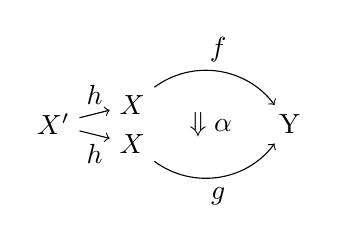
\begin{tikzpicture}
    \node (A) at (0,0) {$X'$};
    \node (B) at (1,0.25) {$X$}
      edge [<-] node [above] {$h$} (A);
    \node (B') at (1,-0.25) {$X$}
      edge [<-] node [below] {$h$} (A);
    \node (C) at (3,0) {Y}
      edge [<-, bend right=45] node [above] {$f$} (B)
      edge [<-, bend left=45] node [below] {$g$} (B');
    \node (D) at (2,0) {$\Downarrow\alpha$};
  \end{tikzpicture}
\end{center}

The lax equalizers in the theory provide a notion of a modal operator.  For example, in the SKI combinator calculus, we can construct the lax equalizer of the context $t, u, v \mapsto (t\; u)$ and the context $t, u, v \mapsto v;$ the result can be thought of as those triples of terms $(t, u, v)$ such that $(t\; u)$ eventually reduces to $v.$  If we restrict to $u \in \llbracket A \rrbracket$ and $v \in \llbracket B \rrbracket,$ then the lax equalizer is effectively the type $A \Rightarrow B.$

\section{Interesting formulae}

\begin{comment}
  * Examples of interesting formulae

      * primes in a monoid

      * deadlock-free (both kinds)

      * datalock-free? http://erights.org/elang/concurrency/epimenides.html

      * deniability from paper with Drossopolou

      * more?  
\end{comment}

[[ Put formulae here. ]]

\section{Combining term calculi}

[[ Anecdote about pi calculus and ambient calculus. ]]

Composing the term calculus monads is one way to combine the calculi; it, too, requires a distributive law.  Given monads $T$ and $T'$ and a distributive law transformation $\Delta\colon T'T \Rightarrow TT'$, we can form a monad $TT'$ where the monadic join is
\[ \mu^{TT'}_X\colon TT'TT'X \xrightarrow{\mu^T_{T'X} \circ TT(\mu^{T'}_X) \circ \Delta_X} TT'X. \]
However, there is often no natural way to produce such a distributive law.

The cartesian product of two 2-theories is a 2-theory representing running two isolated computers in parallel; this is not a particularly interesting way of combining term calculi.

A different approach to combining term calculi is to combine the grammars so that either language may be used within the other.  [[ Coproduct of theories in 2-Law. ]]

\subsubsection{Related work}

%Montanari, et al have considered double category models of the {\pic}.

TBD

\subsubsection{Organization of the rest of the paper}

TBD

%%% ----------------------------------------------------------------------

\section{Some motivating examples}

In this section we motivate the construction by way of a few examples
familiar both to computer scientists and category theorists.



\subsubsection{Varying the collection monad}

TBD

\subsection{A logic for lambda}

TBD

\subsubsection{Some formulae in a logic for lambda}

TBD

\subsection{A categorical rewrite}

In the categorical presentation of the term calculus for monoids,
we use a Lawvere 2-theory \cite{PowerLack, Yanofsky}.  We have a 
sort for terms, morphisms for the term constructors,
rewrite rules for structural equivalence and reduction, and relations
between rewrites.

In particular, we have a Lawvere 2-theory Th(Mon) with one sort 
$T$ for terms; the function symbols
\begin{grammar}
{T[G]} \bc e & \mbox{$e : 1 \to T$} \\
\;\;\; \bm \; g_i & \mbox{$g_i : 1 \to T$} \\
\;\;\; \bm \; T[G] * T[G] & \mbox{$m: T \times T \to T$,} \\
\end{grammar}
corresponding to the term constructors generate a $(G+1)$-pointed magma.

Structural equivalence is interpreted as bi-directional morphisms
$T \to T$. Most programming languages have free monoids built into
the language in the form of lists; some though, like Scheme and Haskell,
use an operator called ``cons'' to build lists out of ordered pairs,
exactly as we are doing with $m$.  In order to compare two
words of a monoid using the constructors above, we have to compute
a normal form.

We arbitrarily choose to have the parentheses at the right 
and no occurrences of $e()$ unless the normal form is $e()$ itself.  
Our rewrite rules are
$$\begin{array}{rll}
a:& ((x\;y)\;z) \Rightarrow (x\;(y\;z))\\
l:& (e()\;x) \Rightarrow x\\
r:& (x\;e()) \Rightarrow x\\
\end{array}$$
Finally, we impose relations on the rewrite rules.  The rewrites
$a,l,$ and $r$ satisfy the pentagon and triangle equations
from a monoidal category.

We can take models in any 2-category with finite products; if we take
models in the category Set thought of as a 2-category, then the
rewrite rules are identities, thus invertible, and we get
monoids generated by at least $G$. If instead we take models in Cat,
we get a category $T$ of words in a $(G+1)$-pointed magma with rewrites 
between them.  Once we begin to consider words with rewrites between
them, we call the words ``processes''.


\subsection{A logic for {\pic}}

\subsubsection{Our running process calculus}

\subsubsection{Syntax}
\label{syntax}
\begin{grammar}
{P} \bc \pzero & \mbox{stopped process} \\
       \;\;\; \bm \; {x}{?}{( y_1, \ldots, y_n )} \Rightarrow {P} & \mbox{input} \\
       \;\;\; \bm \; {x}{!}{( y_1, \ldots, y_n )} & \mbox{output} \\
%       \;\;\; \bm \; {M}{+}{N} & \mbox{choice} \\
%{ P, Q } \bc M & \mbox{include IO processes} \\                                
       \;\;\; \bm \; (\mathsf{new}\; x){P} & \mbox{new channel} \\
       \;\;\; \bm \; {P} \juxtap {Q} & \mbox{parallel} \\                                
\end{grammar}

Due to space limitations we do not treat replication, $!P$.

\subsubsection{Free and bound names}

\begin{equation*}
  \begin{aligned}
    & \freenames{\pzero} \defneqls \emptyset \\
    & \freenames{{x}{?}{( y_1, \ldots, y_n )} \Rightarrow {P}} \defneqls \\
    & \;\;\;\;\;\{ x \} \cup (\freenames{P} \setminus \{ y_1, \ldots y_n \}) \\
    & \freenames{{x}{!}{( y_1, \ldots, y_n )}} \defneqls \{ x, y_1, \ldots, y_n \} \\
    & \freenames{(\mathsf{new}\; x){P}} \defneqls \freenames{P} \setminus \{x\} \\    
    & \freenames{{P} \juxtap {Q}} \defneqls \freenames{P} \cup \freenames{Q} \\
  \end{aligned}
\end{equation*}

An occurrence of $x$ in a process $P$ is \textit{bound} if it is not
free. The set of names occurring in a process (bound or free) is
denoted by $\names{P}$.

\subsubsection{Structural congruence}
\label{congruence}

The {\em structural congruence} of processes, noted $\scong$, is the
least congruence containing $\alpha$-equivalence, $\alphaeq$, making
$( P, |, 0 )$ into commutative monoids and satisfying

\begin{equation*}  
  (\mathsf{new}\; x)(\mathsf{new}\; x){P} \scong (\mathsf{new}\; x)P
\end{equation*}
\begin{equation*}  
  (\mathsf{new}\; x)(\mathsf{new}\; y){P} \scong (\mathsf{new}\; y)(\mathsf{new}\; x)P
\end{equation*}
\begin{equation*}  
  ((\mathsf{new}\; x){P}) \juxtap {Q} \scong (\mathsf{new}\; x)({P} \juxtap {Q})
\end{equation*}

\subsubsection{Operational Semantics}\label{section:opsem}
 
\infrule[Comm]
{ |\vec{y}| = |\vec{z}| }
%{P_1 + {{ x_{0}{?}{(}{\vec{y}}{)} \concat {P}}\juxtap {x_{1}}{!}{(}{\vec{z}}{)} + P_2}
{{{ x{?}{(}{\vec{y}}{)} \concat {P}}\juxtap {x}{!}{(}{\vec{z}}{)}}
\red {{P}{\{}\vec{z}{/}{\vec{y}}{\}}}}

In addition, we have the following context rules:

\infrule[Par]{{P} \red {P}'}{{{P} \juxtap {Q}} \red {{P}' \juxtap {Q}}}

\infrule[New]{{P} \red {P}'}{{(\mathsf{new}\; x){P}} \red {(\mathsf{new}\; x){P}'}}

\infrule[Equiv]{{{P} \scong {P}'} \andalso {{P}' \red {Q}'} \andalso {{Q}' \scong {Q}}}{{P} \red {Q}}

\subsubsection{Bisimulation}

\begin{defn}
An \emph{observation relation}, $\downarrow$ is the smallest relation satisfying the rules
below.

\infrule[Out-barb]{ }
      {{x}!(\vec{y}) \downarrow x}
\infrule[Par-barb]{\mbox{$P\downarrow x$ or $Q\downarrow x$}}
      {\mbox{$P \juxtap Q \downarrow x$}}
\infrule[New-barb]{\mbox{$P\downarrow x$, $x \neq u$}}
      {\mbox{$(\mathsf{new}\; u){P} \downarrow x$}}

% We write $P \Downarrow x$ if there is $Q$ such that 
% $P \wred Q$ and $Q \downarrow x$.
\end{defn}

Notice that $\prefix{x}{y}{P}$ has no barb.  Indeed, in {\pic} as well
as other asynchronous calculi, an observer has no direct means to
detect if a sent message has been received or not.

\begin{defn}
%\label{def.bbisim}
An \emph{barbed bisimulation}, is a symmetric binary relation 
${\mathcal S}$ between agents such that $P\rel{S}Q$ implies:
\begin{enumerate}
\item If $P \red P'$ then $Q \red Q'$ and $P'\rel{S} Q'$.
\item If $P\downarrow x$, then $Q\downarrow x$.
\end{enumerate}
$P$ is barbed bisimilar to $Q$, written
$P \wbbisim Q$, if $P \rel{S} Q$ for some barbed bisimulation ${\mathcal S}$.
\end{defn}

\section{Logic as distributive law}

TBD

\section{Conclusions and future work}

TBD

\paragraph{Acknowledgments}

TBD

% ------------------------------------------------------------------------
%GATHER{Xbib.bib}   % For Gather Purpose Only
%GATHER{Paper.bbl}  % For Gather Purpose Only
\bibliographystyle{amsplain}
\bibliography{ladl}

% ------------------------------------------------------------------------



% ------------------------------------------------------------------------

\end{document}
% ------------------------------------------------------------------------
